% questions.tex —— 2018 年·浙江卷 · 题目内容片段（无答案）
% 由 tools/generate_projects.py 依来源总账自 2018/2018_数学真题_浙江_试题.md 生成，勿手改（改源 MD 后重跑）

\begin{gktip}
来源：固定来源 \texttt{src-1dea114bc61a98aeedb195d0b903e192d79b25f77de513dfd08ca9d3467eac54}（\texttt{普通高考/2018/2018浙江.pdf}，原卷印刷页 1085—1086）。
声明：内部绑定只固定输入字节，不认证出版者、版次、上游来源链及官方身份；固定源不附答案页。
\end{gktip}

\par\medskip

\gkpart{一、选择题（本大题共 10 小题，每小题 4 分，共 40 分。在每小题给出的四个选项中，只有一项是符合题目要求的）}

\begin{question}
\gkti{1}
已知全集 $U = \{1, 2, 3, 4, 5\}$，$A = \{1, 3\}$，则 $\complement_U A =$（ ）。

(A) $\varnothing$　(B) $\{1, 3\}$　(C) $\{2, 4, 5\}$　(D) $\{1, 2, 3, 4, 5\}$

\end{question}
\begin{question}
\gkti{2}
双曲线 $\dfrac{x^2}{3} - y^2 = 1$ 的焦点坐标是（ ）。

(A) $(-\sqrt2, 0), (\sqrt2, 0)$　(B) $(-2, 0), (2, 0)$　(C) $(0, -\sqrt2), (0, \sqrt2)$　(D) $(0, -2), (0, 2)$

\Needspace{0.4\textheight}
\end{question}
\begin{question}
\gkti{3}
某几何体的三视图如图所示（单位：$\mathrm{cm}$），则该几何体的体积（单位：$\mathrm{cm}^3$）是（ ）。
\nopagebreak[4]
\begin{center}% 2018 浙江卷第3题：三视图
\begin{tikzpicture}[font=\small, line cap=round, line join=round, >=stealth]
  % 正视图
  \begin{scope}
    \draw[thick] (0, 0) rectangle (2, 2);
    \draw[thick] (1, 0) -- (1, 2);
    % 尺寸标注
    \draw[<->] (0, -0.2) -- (1, -0.2) node[midway, fill=white, inner sep=1pt] {$1$};
    \draw[<->] (1, -0.2) -- (2, -0.2) node[midway, fill=white, inner sep=1pt] {$1$};
    \draw[<->] (2.2, 0) -- (2.2, 2) node[midway, fill=white, inner sep=1pt] {$2$};
    \node[below=5mm] at (1, 0) {正视图};
  \end{scope}

  % 侧视图
  \begin{scope}[xshift=3.2cm]
    \draw[thick] (0, 0) rectangle (2, 2);
    % 尺寸标注
    \draw[<->] (0, -0.2) -- (2, -0.2) node[midway, fill=white, inner sep=1pt] {$2$};
    \node[below=5mm] at (1, 0) {侧视图};
  \end{scope}

  % 俯视图（位于正视图下方）
  \begin{scope}[yshift=-3.4cm]
    \draw[thick] (0, 2) -- (2, 2) -- (2, 0) -- (1, 0) -- cycle;
    \node[below=3mm] at (1, 0) {俯视图};
  \end{scope}
\end{tikzpicture}
\end{center}
\nopagebreak[4]
(A) $2$　(B) $4$　(C) $6$　(D) $8$

\end{question}
\begin{question}
\gkti{4}
复数 $\dfrac{2}{1 - \mathrm i}$（$\mathrm i$ 为虚数单位）的共轭复数是（ ）。

(A) $1 + \mathrm i$　(B) $1 - \mathrm i$　(C) $-1 + \mathrm i$　(D) $-1 - \mathrm i$

\Needspace{0.4\textheight}
\end{question}
\begin{question}
\gkti{5}
函数 $y = 2^{|x|}\sin 2x$ 的图象可能是（ ）。
\nopagebreak[4]
\begin{center}% 2018 浙江卷第5题：函数图象选项
\begin{tikzpicture}[line cap=round, line join=round, line width=0.6pt, font=\small]

% (A) 偶函数图象
\begin{scope}[shift={(0, 3.2)}, x=0.8cm, y=0.5cm]
  \draw[->] (-3.8, 0) -- (3.8, 0) node[below] {$x$};
  \draw[->] (0, -2.2) -- (0, 3.2) node[left] {$y$};
  \node[below right] at (0, 0) {$O$};
  \draw (-3.14, 0.08) -- (-3.14, -0.08) node[below left] {$-\pi$};
  \draw (3.14, 0.08) -- (3.14, -0.08) node[below right] {$\pi$};
  \begin{scope}
    \clip (-3.6, -2.0) rectangle (3.6, 3.0);
    \draw[thick, domain=-3.5:3.5, samples=120] plot (\x, {2.2 * sin(deg(abs(\x)))});
  \end{scope}
  \node at (0, -2.7) {(A)};
\end{scope}

% (B) 偶函数双峰双谷图象
\begin{scope}[shift={(6.8, 3.2)}, x=0.8cm, y=0.5cm]
  \draw[->] (-3.8, 0) -- (3.8, 0) node[below] {$x$};
  \draw[->] (0, -2.6) -- (0, 3.2) node[left] {$y$};
  \node[below right] at (0, 0) {$O$};
  \draw (-3.14, 0.08) -- (-3.14, -0.08) node[below left] {$-\pi$};
  \draw (3.14, 0.08) -- (3.14, -0.08) node[below right] {$\pi$};
  \begin{scope}
    \clip (-3.6, -2.4) rectangle (3.6, 3.0);
    \draw[thick, domain=-3.5:3.5, samples=120] plot (\x, {1.2 * cos(2*deg(\x)) - 1.2 * abs(\x)/3.14 + 0.3});
  \end{scope}
  \node at (0, -2.7) {(B)};
\end{scope}

% (C) 奇函数单正峰单负谷图象
\begin{scope}[shift={(0, -3.2)}, x=0.8cm, y=0.5cm]
  \draw[->] (-3.8, 0) -- (3.8, 0) node[below] {$x$};
  \draw[->] (0, -2.6) -- (0, 3.2) node[left] {$y$};
  \node[below right] at (0, 0) {$O$};
  \draw (-3.14, 0.08) -- (-3.14, -0.08) node[below left] {$-\pi$};
  \draw (3.14, 0.08) -- (3.14, -0.08) node[below right] {$\pi$};
  \begin{scope}
    \clip (-3.6, -2.4) rectangle (3.6, 3.0);
    \draw[thick, domain=-3.5:3.5, samples=100] plot (\x, {2.0 * sin(deg(\x))});
  \end{scope}
  \node at (0, -2.7) {(C)};
\end{scope}

% (D) 正确选项：y = 2^{|x|} \sin 2x
\begin{scope}[shift={(6.8, -3.2)}, x=0.8cm, y=0.5cm]
  \draw[->] (-3.8, 0) -- (3.8, 0) node[below] {$x$};
  \draw[->] (0, -2.8) -- (0, 3.2) node[left] {$y$};
  \node[below right] at (0, 0) {$O$};
  \draw (-3.14, 0.08) -- (-3.14, -0.08) node[below left] {$-\pi$};
  \draw (3.14, 0.08) -- (3.14, -0.08) node[below right] {$\pi$};
  \begin{scope}
    \clip (-3.6, -2.6) rectangle (3.6, 2.8);
    \draw[thick, domain=-3.4:3.4, samples=140] plot (\x, {0.35 * pow(2, abs(\x)) * sin(2*deg(\x))});
  \end{scope}
  \node at (0, -2.7) {(D)};
\end{scope}

\end{tikzpicture}
\end{center}
\nopagebreak[4]
(A) 见图 (A)　(B) 见图 (B)　(C) 见图 (C)　(D) 见图 (D)

\end{question}
\begin{question}
\gkti{6}
已知平面 $\alpha$，直线 $m, n$ 满足 $m \not\subset \alpha$，$n \subset \alpha$，则“$m \parallel n$”是“$m \parallel \alpha$”的（ ）。

(A) 充分不必要条件　(B) 必要不充分条件　(C) 充分必要条件　(D) 既不充分也不必要条件

\end{question}
\begin{question}
\gkti{7}
\Needspace{5\baselineskip}
设 $0 < p < 1$，随机变量 $\xi$ 的分布列是

\nopagebreak[4]
\[\begin{array}{|c|c|c|c|}
\hline
\xi & 0 & 1 & 2 \\
\hline
P & \dfrac{1-p}{2} & \dfrac12 & \dfrac{p}{2} \\
\hline
\end{array}\]

则当 $p$ 在 $(0, 1)$ 内增大时，（ ）。

(A) $D(\xi)$ 减小　(B) $D(\xi)$ 增大　(C) $D(\xi)$ 先减小后增大　(D) $D(\xi)$ 先增大后减小

\end{question}
\begin{question}
\gkti{8}
已知四棱锥 $S - ABCD$ 的底面是正方形，侧棱长均相等，$E$ 是线段 $AB$ 上的点（不含端点），设 $SE$ 与 $BC$ 所成的角为 $\theta_1$，$SE$ 与平面 $ABCD$ 所成的角为 $\theta_2$，二面角 $S - AB - C$ 的平面角为 $\theta_3$，则（ ）。

(A) $\theta_1 \leqslant \theta_2 \leqslant \theta_3$　(B) $\theta_3 \leqslant \theta_2 \leqslant \theta_1$　(C) $\theta_1 \leqslant \theta_3 \leqslant \theta_2$　(D) $\theta_2 \leqslant \theta_3 \leqslant \theta_1$

\end{question}
\begin{question}
\gkti{9}
已知 $\boldsymbol a, \boldsymbol b, \boldsymbol e$ 是平面向量，$\boldsymbol e$ 是单位向量。若非零向量 $\boldsymbol a$ 与 $\boldsymbol e$ 的夹角为 $\dfrac{\pi}{3}$，向量 $\boldsymbol b$ 满足 $\boldsymbol b^2 - 4\boldsymbol e \cdot \boldsymbol b + 3 = 0$，则 $|\boldsymbol a - \boldsymbol b|$ 的最小值是（ ）。

(A) $\sqrt3 - 1$　(B) $\sqrt3 + 1$　(C) $2$　(D) $2 - \sqrt3$

\end{question}
\begin{question}
\gkti{10}
已知 $a_1, a_2, a_3, a_4$ 成等比数列，且 $a_1 + a_2 + a_3 + a_4 = \ln(a_1 + a_2 + a_3)$。若 $a_1 > 1$，则（ ）。

(A) $a_1 < a_3, a_2 < a_4$　(B) $a_1 > a_3, a_2 < a_4$　(C) $a_1 < a_3, a_2 > a_4$　(D) $a_1 > a_3, a_2 > a_4$

\par\medskip

\end{question}
\gkpart{二、填空题（本大题共 7 小题，多空题每题 6 分，单空题每题 4 分，共 36 分）}

\begin{question}
\gkti{11}
\Needspace{5\baselineskip}
我国古代数学著作《张邱建算经》中记载百鸡问题：“今有鸡翁一，值钱五；鸡母一，值钱三；鸡雏三，值钱一。凡百钱，买鸡百只，问鸡翁、母、雏各几何？”设鸡翁，鸡母，鸡雏个数分别为 $x, y, z$，则
\nopagebreak[4]
\[\begin{cases} x + y + z = 100, \\ 5x + 3y + \dfrac13 z = 100, \end{cases}\]
当 $z = 81$ 时，$x =$ \underline{\hspace{2cm}}，$y =$ \underline{\hspace{2cm}}。

\end{question}
\begin{question}
\gkti{12}
\Needspace{5\baselineskip}
若 $x, y$ 满足约束条件
\nopagebreak[4]
\[\begin{cases} x - y \geqslant 0, \\ 2x + y \leqslant 6, \\ x + y \geqslant 2, \end{cases}\]
则 $z = x + 3y$ 的最小值是 \underline{\hspace{2cm}}，最大值是 \underline{\hspace{2cm}}。

\end{question}
\begin{question}
\gkti{13}
在 $\triangle ABC$ 中，角 $A, B, C$ 所对的边分别为 $a, b, c$。若 $a = \sqrt7$，$b = 2$，$A = 60^\circ$，则 $\sin B =$ \underline{\hspace{2cm}}，$c =$ \underline{\hspace{2cm}}。

\end{question}
\begin{question}
\gkti{14}
二项式 $\left(\sqrt[3]{x} + \dfrac{1}{2x}\right)^8$ 的展开式的常数项是 \underline{\hspace{2cm}}。

\end{question}
\begin{question}
\gkti{15}
已知 $\lambda \in \mathbf R$，函数 $f(x) = \begin{cases} x - 4, & x \geqslant \lambda, \\ x^2 - 4x + 3, & x < \lambda, \end{cases}$ 当 $\lambda = 2$ 时，不等式 $f(x) < 0$ 的解集是 \underline{\hspace{2cm}}。若函数 $f(x)$ 恰有 $2$ 个零点，则 $\lambda$ 的取值范围是 \underline{\hspace{2cm}}。

\end{question}
\begin{question}
\gkti{16}
从 $1, 3, 5, 7, 9$ 中任取 $2$ 个数字，从 $0, 2, 4, 6$ 中任取 $2$ 个数字，一共可以组成 \underline{\hspace{2cm}} 个没有重复数字的四位数。（用数字作答）

\end{question}
\begin{question}
\gkti{17}
已知点 $P(0, 1)$，椭圆 $\dfrac{x^2}{4} + y^2 = m\ (m > 1)$ 上两点 $A, B$ 满足 $\overrightarrow{AP} = 2\overrightarrow{PB}$，则当 $m =$ \underline{\hspace{2cm}} 时，点 $B$ 横坐标的绝对值最大。

\par\medskip

\end{question}
\gkpart{三、解答题（本大题共 5 小题，共 74 分。解答应写出文字说明、证明过程或演算步骤）}

\begin{question}
\gkti{18}\textbf{（本小题满分 14 分）} 
已知角 $\alpha$ 的顶点与原点 $O$ 重合，始边与 $x$ 轴的非负半轴重合，它的终边过点 $P\left(-\dfrac35, -\dfrac45\right)$。
(1) 求 $\sin(\alpha + \pi)$ 的值；
(2) 若角 $\beta$ 满足 $\sin(\alpha + \beta) = \dfrac{5}{13}$，求 $\cos\beta$ 的值。

\Needspace{0.4\textheight}
\end{question}
\begin{question}
\gkti{19}\textbf{（本小题满分 15 分）} 
如图，已知多面体 $ABCA_1B_1C_1$，$A_1A, B_1B, C_1C$ 均垂直于平面 $ABC$，$\angle ABC = 120^\circ$，$A_1A = 4$，$C_1C = 1$，$AB = BC = B_1B = 2$。
\nopagebreak[4]
\begin{center}% 2018 浙江卷第19题：多面体立体几何示意图
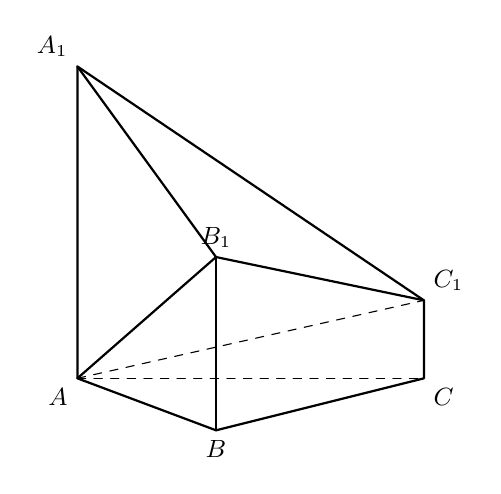
\begin{tikzpicture}[font=\small, line cap=round, line join=round, >=stealth, scale=1.1]
  % 顶点定义
  \coordinate (A) at (0, 0);
  \coordinate (B) at (1.6, -0.6);
  \coordinate (C) at (4.0, 0);
  \coordinate (A1) at (0, 3.6);
  \coordinate (B1) at (1.6, 1.4);
  \coordinate (C1) at (4.0, 0.9);

  % 虚线（隐藏棱）
  \draw[dashed, thin] (A) -- (C);
  \draw[dashed, thin] (A) -- (C1);

  % 实线（可见棱）
  \draw[thick] (A1) -- (A) -- (B) -- (C) -- (C1) -- cycle;
  \draw[thick] (B) -- (B1);
  \draw[thick] (A1) -- (B1) -- (C1);
  \draw[thick] (A) -- (B1);

  % 顶点标签
  \node[above left] at (A1) {$A_1$};
  \node[above] at (B1) {$B_1$};
  \node[above right] at (C1) {$C_1$};
  \node[below left] at (A) {$A$};
  \node[below] at (B) {$B$};
  \node[below right] at (C) {$C$};
\end{tikzpicture}
\end{center}
\nopagebreak[4]
(1) 证明：$AB_1 \perp$ 平面 $A_1B_1C_1$；
(2) 求直线 $AC_1$ 与平面 $ABB_1$ 所成的角的正弦值。

\end{question}
\begin{question}
\gkti{20}\textbf{（本小题满分 15 分）} 
已知等比数列 $\{a_n\}$ 的公比 $q > 1$，且 $a_3 + a_4 + a_5 = 28$，$a_4 + 2$ 是 $a_3, a_5$ 的等差中项。数列 $\{b_n\}$ 满足 $b_1 = 1$，数列 $\{(b_{n+1} - b_n)a_n\}$ 的前 $n$ 项和为 $2n^2 + n$。
(1) 求 $q$ 的值；
(2) 求数列 $\{b_n\}$ 的通项公式。

\Needspace{0.4\textheight}
\end{question}
\begin{question}
\gkti{21}\textbf{（本小题满分 15 分）} 
如图，已知点 $P$ 是 $y$ 轴左侧（不含 $y$ 轴）一点，抛物线 $C\colon y^2 = 4x$ 上存在不同的两点 $A, B$ 满足 $PA, PB$ 的中点均在 $C$ 上。
\nopagebreak[4]
\begin{center}% 2018 浙江卷第21题：抛物线弦中点几何图
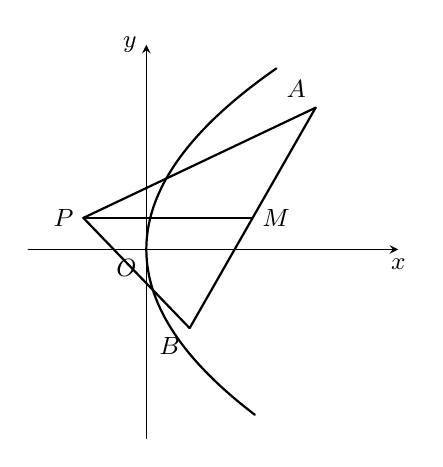
\begin{tikzpicture}[font=\small, line cap=round, line join=round, >=stealth, scale=1.0]
  % 坐标轴
  \draw[->] (-1.5, 0) -- (3.2, 0) node[below] {$x$};
  \draw[->] (0, -2.4) -- (0, 2.6) node[left] {$y$};
  \node[below left] at (0, 0) {$O$};

  % 抛物线 y^2 = 3.5x (示意)
  \draw[thick, domain=-2.1:2.3, samples=90] plot ({(\x)^2 / 3.2}, \x);

  % 关键点定义
  \coordinate (P) at (-0.8, 0.4);
  \coordinate (M) at (1.35, 0.4);
  \coordinate (A) at (2.15, 1.8);
  \coordinate (B) at (0.55, -1.0);

  % 连线
  \draw[thick] (P) -- (M);
  \draw[thick] (A) -- (B);
  \draw[thick] (P) -- (A);
  \draw[thick] (P) -- (B);

  % 标签
  \node[left] at (P) {$P$};
  \node[right] at (M) {$M$};
  \node[above left] at (A) {$A$};
  \node[below left] at (B) {$B$};
\end{tikzpicture}
\end{center}
\nopagebreak[4]
(1) 设 $AB$ 中点为 $M$，证明：$PM$ 垂直于 $y$ 轴；
(2) 若 $P$ 是半椭圆 $x^2 + \dfrac{y^2}{4} = 1\ (x < 0)$ 上的动点，求 $\triangle PAB$ 面积的取值范围。

\end{question}
\begin{question}
\gkti{22}\textbf{（本小题满分 15 分）} 
已知函数 $f(x) = \sqrt x - \ln x$。
(1) 若 $f(x)$ 在 $x = x_1, x_2\ (x_1 \neq x_2)$ 处导数相等，证明：$f(x_1) + f(x_2) > 8 - 8\ln 2$；
(2) 若 $a \leqslant 3 - 4\ln 2$，证明：对于任意 $k > 0$，直线 $y = kx + a$ 与曲线 $y = f(x)$ 有唯一公共点。

\end{question}